
\noindent This chapter covers the following ideas.

\begin{enumerate}

\item Explain the connection between vector fields and their corresponding eigenvalues and eigenvectors. Use this knowledge to apply the second derivative test.
\item Solve various problems relating to conservation laws, including stoichiometry, Kirchoff's electrical laws, and Markov Processes.
\item Use Cramer's rule to solve systems, and explain when you would choose Cramer's rule over row reduction.
\item Find interpolating polynomials, and use the transpose to solve the least squares regression problem.
\item Find the partial fraction decomposition of a rational function. Utilize this decomposition to integrate rational functions.
\item Be able to show that a function is linear, and find the kernel of a linear function. 
\end{enumerate}

\section{Vector Fields}
In multivariate calculus, we studied vector fields of the form $\vec F(x,y) = (M,N)$, where $M$ and $N$ are functions of $x$ and $y$. The derivative of the vector field is the square matrix
$$D\vec F(x,y) =
\begin{bmatrix}
\partial M/\partial x &
\partial M/\partial y \\
\partial N/\partial x &
\partial N/\partial y 
\end{bmatrix}.
$$ 
The eigenvalues and eigenvectors of this matrix provide us with a wealth of information about the vector field.  The next few problems have you discover many of these key ideas.  We'll return to these ideas throughout the semester, especially when we start studying systems of differential equations in depth.

\begin{problem}
Consider the vector field $\vec F(x,y) = (2x+y, x+2y)$. 
\begin{enumerate}
 \item At each of the 8 points given by $(\pm 1, \pm 1)$, $(0, \pm 1)$, $(\pm 1, 0)$, sketch the vector $\vec F(x,y)$ with it's base at the input point (so at point $(1,0)$, sketch $(2,1)$, a vector starting at $(1,0)$ and ending at $(3,1)$).  This provides us with a rough sketch of the vector field.
 \item Compute $A=D\vec F(x,y)$. It should be a 2 by 2 matrix. 
 \item Remember that we say a vector $\vec x$ is an eigenvector if $A\vec x = \lambda \vec x$.  For any of the vectors from part 1., did you find that $A\vec x = \lambda \vec x$?  Which ones (these are eigenvectors)?  By how much was the vector $\vec x$ stretched (these are eigenvalues)? 
 \item Now compute the eigenvalues and eigenvectors of this matrix, using the algorithm from the previous chapter.  You should obtain the same answer as part 3.
\end{enumerate}
\end{problem}

The problem above had two positive eigenvalues. In the next problem, your goal is to determine what a vector field looks like when you have both a positive and negative eigenvalue.

\begin{problem}
Complete the following:
\begin{enumerate}
 \item For the vector field $\vec F = (x, 2x-y)$, compute the eigenvalues and eigenvectors of $D\vec F(x,y)$. 
 \item For the vector field $\vec F = (x-4y, -6x-y)$, compute the eigenvalues and eigenvectors of $D\vec F(x,y)$. 
 \item With each vector field, use a computer to construct a vector field plot.  In the plot, please show us how to see the eigenvectors, together with which eigenvector corresponds to a positive eigenvalues, and which corresponds to a negative eigenvalue. You can construct vector fields in Wolfram|Alpha by typing ``vector field plot'' in the input box, or just  follow the link \url{http://www.wolframalpha.com/input/?i=vector+field+plot&lk=4&num=2}.
 \item Add to your plots several trajectories, i.e. a path that a particle would follow if $\vec F$ represents the tangent vectors of the path.  Think, ``If I dropped a really light particle in this field, representing water current, where would the particle go? \note{adding an example here could help them, that way they know what they are doing.  A link to an appropriate vector field plot would do it.}
\end{enumerate}
\end{problem}

\begin{problem}
The following three vector fields have imaginary eigenvalues. Compute the eigenvalues for each, construct a vector field plot, and on the plot add several trajectories (the path followed by a particle that is dropped into this field).
\begin{enumerate}
 \item $\vec F = (-2y,x)$. 
 \item $\vec F = (-x+y, -x-y)$.
 \item $\vec F = (x-y, x)$ 
\end{enumerate}
Make a conjecture as to why one spirals in, one spirals out, and one just wraps around in ellipses. We'll address this conjecture in class.
\end{problem}

The next problem requires that you are on a computer that can use Mathematica. These computers are available in the Ricks, Austin, Romney, and library.  Alternately, you can download VMWare that will allow you to use Mathematica for free from your computer, provided you head to \url{https://vdiview.byui.edu/}. You can download step-by-step instructions from \url{http://www.byui.edu/help-desk/categories/vdivmware}. Please take a moment and make sure you can access Mathematica.

\begin{problem}
Start by downloading the Mathematica notebook \href{https://www.dropbox.com/s/1df1nswgbq3y34n/316-VectorField.nb}{VectorFields.nb (click on the link)}.  The goal of this problem is to make a connection between a vector field and it's corresponding eigenvalues/eigenvectors. Once the notebook is open, click somewhere in the text, hold down Shift, and then press Enter.  This will evaluate the commands and produce a vector field plot, with the eigenvector directions drawn in green. You can click on the bubbles with crosshairs in them to adjust the vectors (which are the columns of the matrix). Play around with the animation until you feel like you can answer each of the following questions.
 \begin{enumerate}
  \item If the vector field pushes things outwards in all directions, what do you know about the eigenvalues?
  \item If the vector field pulls things inwards in all directions, what do you know about the eigenvalues?
  \item How can you tell, by looking at a vector field plot, that one eigenvalue is positive and the other is negative?
  \item If the vector field involves swirling motion, what do you know about the eigenvalues? What makes the difference between spiraling inwards, outwards, or just spinning in circles?
  \item What happens when you have a repeated eigenvalue? This one has lots of correct answers, and it a topic for much further discussion in chapter 10. See if you can get an example of a repeated eigenvalue with a behavior that's different from the above. If you have the first 4, you can present in class. We'll have you come up to the computer and show us what you did.
 \end{enumerate}
\end{problem}


\subsection{Second Derivative Test}

Vector fields and eigenvalues provide us with precisely the key information needed to locate maximums, minimums, and saddles for functions of the form $z=f(x,y)$. 

\begin{problem}
 Consider the function $f(x,y)= x^2+4xy+y^2$. The derivative (gradient) is the vector field $Df(x,y) = (2x+4y,4x+2y)$. See Figure \ref{second derivative graph} for a graph of several level curves, together with the gradient.
\begin{enumerate}
\item At what point(s) does $Df(x,y)=\vec 0$? These are the potential locations of maximums, minimums, or saddles.   
\item Compute the second derivative of $f$, which should give you a 2 by 2 symmetric matrix. This matrix is called the Hessian.
\item By looking at the picture, are the eigenvalues of $D^2f(x,y)$ both positive, both negative, or do they differ in sign?  How can you tell? Then confirm you are correct by computing the eigenvalues and eigenvectors of $D^2f(x,y)$.  
\item Recall that the gradient points in the direction of greatest increase.  Using this information alone, does the function have a maximum, minimum, or saddle point at $(x,y)=(0,0)$
\end{enumerate}


\begin{figure}
 \begin{center}\includegraphics{second-derivative-test}\end{center}
\caption{A plot of several level curves of $f(x,y)=x^2+4xy+y^2$ and the gradient. In one direction the gradient is pulling things towards the origin.  In another direction, the gradient is pushing things away from the origin. \label{second derivative graph}}
\end{figure}
\end{problem}
 
\begin{theorem}
 Let $f(x,y)$ be a function that is twice continuously differentiable. Suppose that $Df(x,y)=(0,0)$ when $(x,y)=(a,b)$, so that $(a,b)$ is a critical point. To determine if the point $(a,b)$ corresponds to a maximum, minimum, or saddle point, we compute the eigenvalues of $D^2f(a,b)$ (the second derivative is called the Hessian).
\begin{itemize}
 \item If the eigenvalues of $a$ are all positive, then the function has a minimum at $(a,b)$. 
 \item If the eigenvalues of $a$ are all negative, then the function has a maximum at $(a,b)$. 
 \item If there is a positive eigenvalue, and a negative eigenvalue, then the function has a saddle at $(a,b)$. 
 \item If zero is an eigenvalue, then the second derivative test fails.
\end{itemize}
\end{theorem}

\begin{problem}
 Consider the function $f(x,y) = x^3 - 3x ^2 - y^2 + 2y$
See Figure \ref{second derivative graph2} for a graph of several level curves, together with the gradient.
\begin{enumerate}
\item At what point(s) does $Df(x,y)=\vec 0$? You should obtain two points. These are the potential locations of maximums, minimums, or saddles.   
\item Compute the second derivative of $f$, which should give you a 2 by 2 symmetric matrix. 
\item Pick one of the critical points. Use the vector field plot to decide if the eigenvalues of $D^2f(x,y)$ both positive, both negative, or differ in sign at that critical point, and if the function has a maximum, minimum, or saddle at that point.  Then repeat with the other critical point. 
\item Now compute the eigenvalues of the Hessian at each critical value. This should confirm your answer to part 3. (The matrix is diagonal, so computing eigenvalues should be quick.)  
\end{enumerate}

\begin{figure}
 \begin{center}\includegraphics{second-derivative-test2}\end{center}
\caption{A plot of several level curves of $f(x,y)=x^3-3x^2-y^2+2y$ and the gradient. There are two critical points.  The vector field plot provides enough information to determine if the sign of the eigenvectors of the second derivative at each critical point. \label{second derivative graph2}}
\end{figure}
\end{problem}

The following example adds a little more information to this discussion. I've included it to give you one additional piece of information, namely how the eigenvalues connect to the concavity of the function. 

\begin{example}
For the function {$f(x,y)=x^2+xy+y^2$}, the gradient is $Df = \begin{bmatrix}2x+y&x+2y \end{bmatrix}$, which is zero only at $x=0,y=0$ (solve the system of equations $2x+y=0,x+2y=0$). The Hessian is $D^2f = \begin{bmatrix}2&1 \\1&2\end{bmatrix}$. The eigenvalues are found by solving $0=\det \begin{bmatrix}2-\lambda &1 \\1&2-\lambda \end{bmatrix} = (2-\lambda)^2-1 = 4-4\lambda+\lambda^2 -1 = (\lambda-3)(\lambda-1)$, so $\lambda = 3,1$ are the eigenvalues.  Since both eigenvalues are positive, the gradient pushes things away from the origin in all direction, which means in every direction you move from the critical point, you'll increase in height.  There is a minimum at $(0,0)$.  

The eigenvectors of the Hessian help us understand more about the graph of the function.  An eigenvector corresponding to 3 is $(1,1)$, and corresponding to 1 is $(-1,1)$. These vectors are drawn in figure \ref{2ndder}, together with two parabolas whose 2nd derivatives are precisely 3 and 1.  The parabola which opens upwards the most quickly has a 2nd derivative of 3.  The other parabola has a second derivative of 1. In every other direction, the 2nd derivative would be between 1 and 3.
\end{example}

%\marginpar{{
\begin{figure}[ht
]\begin{center}
\includegraphics[width=2in]{support/2nddertest1}
\hspace{.5in}
\includegraphics[width=2in]{support/2nddertest2}
\end{center}
\caption{The eigenvectors of the second derivative tell you the directions in which the 2nd derivative is largest and smallest. At each critical point, two eigenvectors are drawn as well as a parabola whose second derivative (the eigenvalue) matches the second derivative of the surface in the corresponding eigenvector direction.}
\label{2ndder}
\end{figure}
%}}


\section{Conservation Laws}
Many problems in nature arise from conservation laws.  These laws generally focus on the principle that matter is neither is created nor destroyed, rather it is just moved, changed, or something.  Any of the following could be viewed as a conservation law:
\begin{itemize}
 \item What comes in must come out.
 \item Voltage supplied equals voltage suppressed.
 \item Atoms before equal atoms after.
 \item The change in a quantity is how much it increases minus how much it decreases.
 \item Current in equals current out.
\end{itemize}
The following problems related to some conservation law.  You'll see similar laws in your future classes, regardless of your discipline.


\subsection{Stoichiometry}
Chemical reaction stoichiometry is the study balancing chemical equations. A chemical reaction will often transform reactants into by-products. The by products are generally different compounds, together with either an increase or decrease in heat. One key rule in stoichiometry is that a chemical process neither creates nor destroys matter, rather it only changes the way the matter is organized. For simple reactions (with no radioactive decay), this conservation law forces the number of atoms entering a reaction to be the same as the number leaving. The next problem asks you to use this conservation law to create a balanced chemical reaction equation. 
\begin{problem}
 The chemical compound hydrocarbon dodecane ($C_{12}H_{26}$) is used as a jet fuel surrogate (see Wikipedia for more info).  This compound reacts with oxygen $(0_2)$, and the chemical reaction produces carbon dioxide ($CO_2$), water ($H_2 0$), and heat.  Suppose we expose some dodecane to oxygen, and that a chemical reaction occurs in which the dodecane is completely converted to carbon dioxide and water.  
 Conservation requires that the number of atoms ($H$, $C$, and $0$) at the beginning of the chemical reaction must be the exact same as the number at the end. 
 We could write the chemical reaction in terms of molecules as
 $$x_1 C_{12}H_{26} +x_2 O_2 = x_3 CO_2+ x_4 H_2O\quad \text{or} \quad x_1 C_{12}H_{26} -x_2 O_2 = x_3 CO_2- x_4 H_2O=0, $$
 where $x_1$ molecules of dodecane and $x_2$ molecules of oxygen were converted to $x_3$ units of carbon dioxide and $x_4$ units of oxygen.  
 If we look at each atom (carbon, hydrogen, and oxygen) individually, we obtain three equations to relate the variables $x_1, x_2, x_3, x_4$.  The carbon equation is simply
 $$x_1(12) + x_2(0) = x_3(1)+x_4(0) \quad \text{or}\quad x_1(12) + x_2(0) - x_3(1)-x_4(0)=0.$$  
 Your job follows:
\begin{enumerate}
 \item Write the other two conservation equations (for hydrogen and oxygen). 
 \item Solve the corresponding system of equations by row reduction.  As there are only 3 equations with 4 unknowns, you should obtain infinitely many solutions. Write each variable in terms of the free variable.  
 \item If about 10,000 molecules of water are present at the end of the reaction, about how many molecules of dodecane were burned? 
\end{enumerate}
\end{problem}





\subsection{Kirchoff's Electrical Laws}
Gustav Kirchoff discovered two laws of electricity that pertain to the conservation of charge and energy.  To describe these laws, we must first discuss voltage, resistance, and current.  
\begin{itemize}
 \item Current is the flow of electricity, and often it can be compared to the flow of water.  
 \item As a current passes across a conductor, it encounters resistance. Ohm's law states that the product of the resistance $R$ and current $I$ across a conductor equals the voltage $V$, i.e. $RI=V$. If the voltage remains constant, then a large resistance corresponds to a small current. 
 \item A resistor is an object with high resistance which is placed in an electrical system to slow down the flow (current) of electricity.  Resistors are measured in terms of ohms, and the larger the ohms, the smaller the current.   
\end{itemize}
Figure \ref{ecir} illustrates two introductory electrical systems.
\begin{figure}[htb]
\begin{center}
\begin{tabular}{cc}
\input{electric-circuit-2-loops}
&
\input{electric-circuit-3-loops}
\\
Two Loop System & Three Loop System
\end{tabular}\end{center}
\caption{Electrical Circuit Diagrams.\label{ecir}}
\end{figure}
In this diagram, wires meet at nodes (illustrated with a dot).  
Batteries and voltage sources (represented by 
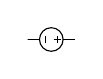
\begin{tikzpicture}[scale=.15,rotate=-90]
%	\useasboundingbox (-.5,-3) rectangle (.5,3);
	\clip (-1,-2) rectangle (1,2);
	\draw (0,0) circle (1cm);
	\draw (.3,.5) -- (-.3,.5);
	\draw (0,.2) -- (0,.8);
	\draw (.3,-.5) -- (-.3,-.5);
	\draw (0,1) -- (0,3);
	\draw (0,-1) -- (0,-3);
\end{tikzpicture}
or other symbols)
supply a voltage of $E$ volts.  At each node the current may change, so the arrows and letters $i$ represent the different currents in the electrical system. The electrical current on each wire may or may not follow the arrows drawn (a negative current means that the current flows opposite the arrow). Resistors are depicted with the symbol 	
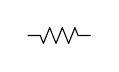
\begin{tikzpicture}[scale=.2,rotate=90]
%	\useasboundingbox (0,-3) rectangle (0,3);
	\clip (-.5,-2) rectangle (.5,2);
	\draw (0,-3) -- ++(0,1.8) -- ++(.5,.2) 
		-- ++(-1,.4) -- ++(1,.4)
		-- ++(-1,.4) -- ++(1,.4)
		-- ++(-1,.4) -- ++(.5,.2)
		-- ++(0,1.8) ;
	\end{tikzpicture}
, and the letter $R$ represents the ohms. 

Kirchoff discovered two laws. They both help us find current in a system, provided we know the voltage of any batteries, and the resistance of any resistors. 
\begin{enumerate}
	\item Kirchoff's current law states that at every node, the current flowing in equals the current flowing out (at nodes, current in = current out). 
	\item Kirchoff's voltage law states that on any loop in the system, the directed sum of voltages supplied equals the directed sum of voltage drops (in loops, voltage in = voltage out). To use this law, pick a spot in the system.  Then move around the system following a path that eventually gets you back to where you began (a closed curve). If you encounter a battery (a voltage source), then it counts as voltage in.  If you encounter a resistor as you move with the current, then the voltage drop is $Ri$.  If you encounter a resistor while moving opposite the current, then times by a negative to get a voltage drop of $-R_i$.
\end{enumerate}

Let's use Kirchoff's laws to generate a system of equations for the two loop system. Remember that every time a current encounters a resistor, the voltage drop is $V=RI$, the product of the resistance and the current. 
\begin{problem} \label{kirchoff 2 loop general}
Consider the two loop system in figure \ref{ecir}. Assume that the voltage supplied from the battery $E$, as well as the ohms $R_1$, $R_2$, and $R_3$, on the resistors are known. The currents $i_1$, $i_2$, and $i_3$ are unknown.
\begin{enumerate}
 \item Use Kirchoff's laws to explain how to obtain each of the equations below:
$$
\begin{array}{rl}
i_1-i_2-i_3&=0\\
-i_1+i_2+i_3&=0\\
R_1i_1+R_2i_2&=E\\
-R_2 i_2 +R_3i_3&=0.\\
R_1i_1 + R_3i_3&=E.
\end{array}
$$
[Hint: If you encounter a resistor while moving backwards along a loop, then times the voltage drop becomes a voltage gain (times by a negative).]
 \item Some of the equations above are linear combinations of the other equations.  How could you obtain the 2nd and 5th as a linear combination of the others?
 \item If $E = 12$, $R_1 = 2$, $R2 = 3$, and  $R3 = 6$, then solve the system of equations above by row reducing an appropriate matrix.    
\end{enumerate}
\end{problem}

\begin{problem}
Consider the three loop system in figure \ref{ecir}. Assume that the voltage supplied from the battery $E$ and that the ohms $R_j$ on the resistors are known. The currents are unknown.
\begin{enumerate}
 \item There are 4 nodes in this system. Write the 4 equations we obtain by remember that the flow in at a node must equal the flow out. 
 \item There are three inner loops in the system above. Write the equations formed by going around each inner loop. [To get an inner loop, pick any point in the system. Then move in a clockwise fashion around the loop
 \item Some of the equations above are linear combinations of the other equations.  How could you obtain the 2nd and 5th as a linear combination of the others?
 \item Why will row reducing the following matrix give you the unknown currents? 
$$\begin{bmatrix}[llllll|l]
 1 & -1 & -1 & 0 & 0 & 0 & 0 \\
 0 & 0 & 1 & -1 & -1 & 0 & 0 \\
 0 & 0 & 0 & 1 & 1 & -1 & 0 \\
 R_1 & R_2 & 0 & 0 & 0 & 0 & E \\
 0 & -R_2 & R_3 & R_4 & 0 & R_6 & 0 \\
 0 & 0 & 0 & -R_4 & R_5 & 0 & 0
\end{bmatrix}.$$
[Don't row reduce this matrix.]
\end{enumerate}
\end{problem}


\begin{problem}
 Consider the three loop system in figure \ref{ecir}. If $E = 12$, $R1 = 1$, $R2 = 1$, $R3 = 1$, $R4 = 1$, $R5 = 1$, $R6 = 1$
 then find the unknown currents by row reducing the matrix in part 4 above. Use a computer to check your answer.  The row reduction is quite short, because the matrix is sparse (has lots of zeros).]
\end{problem}







\subsection{Markov Processes}
Matrices can be used to model a process called a Markov Process. To fit this kind of model, a process must have specific states, and the matrix which models the process is a transition matrix which specifies how each state will change through a given transition. An example of a set of states is ``open'' or ``closed'' in an electrical circuit, or ``working properly'' and ``working improperly'' for operation of machinery at a manufacturing facility. A car rental company which rents vehicles in different locations can use a Markov Process to keep track of where their inventory of cars will be in the future. Stock market analysts use Markov processes and a generalization called stochastic processes to make predictions about future stock values.

\begin{problem}
Suppose we own a car rental company which rents cars in Idaho Falls and Rexburg. The last few weeks have shown a weekly trend that 60\% of the cars which are rented in Rexburg will remain in Rexburg (the other 40\% end up in Idaho Falls). About 80\% of the cars which are rented in Idaho Falls will remain in Idaho Falls (the other 20\% end up in Rexburg). 
\begin{enumerate}
 \item If there are currently 60 cars in Rexburg and 140 cars in IF, how many will be in each city next week? In two weeks?
 \item Let $R_n$ and $I_n$ be the number of cars in Rexburg and Idaho Falls, respectively, at the beginning of the $n$th week (so $R_0=60$ and $I_0=140$). Obtain a matrix $A$ so that $A\pvec{R_0\\I_0} = \pvec{R_1\\I_1}$.  Then check that $A\pvec{R_1\\I_1} = \pvec{R_2\\I_2}$.
 \item We would like to know if the number of cars will stabilize in each city. This would mean that if the current week's car totals are $R$ and $I$, then we could find the next week's totals by solving the system $$A\pvec{R\\I} = \pvec{R\\I},$$  the totals don't change. This is called a steady state solution. Find the steady state solution.  
 \item In the long run, what proportion of the cars will end up in Rexburg?
 \item Because the system $A\pvec{R\\I} = \pvec{R\\I}$ had a nonzero solution, we know something about the eigenvalues of the matrix $A$.  What is an eigenvalue of $A$?
\end{enumerate}
(We'll answer 4 and 5 in class if you are unable.  The key parts are 1-3.) 
\end{problem}

The matrix $A$ found above is called a transition matrix.  It's the matrix which tells you how to move from the current state $\vec x_n$ to the next state $\vec x_{n+1}$. This means we have 
\begin{align*}
\vec x_1 &= A\vec x_0\\
\vec x_2 &= A\vec x_1 = A(A\vec x_0) = A^2\vec x_0\\
\vec x_3 &= A\vec x_2 = A(A\vec x_1) =\cdots = A^3\vec x_0\\
\vec x_4 &= A\vec x_3 = A(A\vec x_2) =\cdots = A^4\vec x_0\\
&\vdots
\end{align*}
You can find the $n$th state by computing $\vec x_n = A^n \vec x_0$, just raise the matrix to a power, and times by the initial state. Let's use this idea once more.

\begin{problem}
In a certain town, there are 3 types of land zones: residential, commercial, and industrial. 
The city has been undergoing growth recently, and the city has noticed the following 5 year trends.  
\begin{itemize}
 \item Every 5 years, they've notice that 10\% of the residential land gets rezoned as commercial land, while 5\% of the residential land gets rezoned as industrial.  The other 85\% of residential land remains residential.  
 \item For commercial land, 70\% remains commercial, while 10\% becomes residential and 20\% becomes industrial. 
 \item For industrial land, 60\% remains industrial, while 25\% becomes commercial and 15\% becomes residential. 
 \item Currently the percent of land in each zone is 40\% residential, 30\% commercial, and 30\% industrial. 
\end{itemize}
Let's assume that these trends continue over an extended period of time.  
\begin{enumerate}
 \item The current state is $\vec x_0 = (40,30,30)$. After 5 years, what percentage of land will be zoned residential? Commercial? Industrial?  Answering this question should give you the transition matrix $A$ so that $\vec x_1=A\vec x_0$. 
 \item Use software to find $\vec x_2$, $\vec x_3$, and $\vec x_4$ (the land use percentages after 10, 15, and 20 years).  
 \item Find the steady state solution to this Markov Process by solving $A\vec x = 1\vec x$ (i.e., the eigenvector corresponding to the eigenvalue $\lambda =1$.)
\end{enumerate}
\end{problem}


\begin{problem}
Consider three occupations, farming, manufacturing, and clothing.  Assume that goods are exchanged between the communities through barter only. Here is how the communities exchange their goods.
\begin{itemize}
 \item The farming community keeps 1/2 of their goods, giving 1/4 to manufacturing and 1/4 to clothing.
 \item The manufacturing community keeps 1/3 of their goods, giving 1/3 to farming and 1/3 to clothing.
 \item The clothing community keeps 1/4 of their goods, giving 1/2 to farming and 1/4 to manufacturing.
\end{itemize}
Answer the following questions.
\begin{enumerate}
\item Suppose that all the commodities have the exact same value.  If each group starts out with 12 units of their commodity, then after 1 round of bartering, how many units will each group have?  Along the way you should produce a transition matrix $A$ so that $A\pvec{12\\12\\12}$ gives the answer.
\item Let $x_1$ be the value of the goods produced by farming. Let $x_2$ be the value of the goods produced by manufacturing. Let $x_3$ be the value of the goods produced by clothing.   We would like to assign a value to each commodity so that each group gets a fair deal when they barter.  To do this, we need to have the value of goods obtained after bartering to match the value of the goods obtained before.  Explain why we can obtain this by solving the equations
$$\begin{bmatrix}
   \frac{1}{2}& \frac{1}{3}& \frac{1}{2}\\
   \frac{1}{4}& \frac{1}{3}& \frac{1}{4}\\
   \frac{1}{4}& \frac{1}{3}& \frac{1}{4}
  \end{bmatrix}
\begin{bmatrix}
 x_1\\x_2\\x_3
\end{bmatrix}
=
\begin{bmatrix}
 x_1\\x_2\\x_3
\end{bmatrix}.
$$  
Then solve this equation.
\item  (We'll answer this one in class.  Try to come up with an answer yourself.) 
If the value of commodities from each group is the same, who is getting the better deal?  To make sure bartering results in a fair deal for all, should farming commodities be more expensive, or less expensive than the others? 
\end{enumerate}
\end{problem}




\section{Cramer's Rule}
Gabriel Cramer developed a way to solve linear systems of equations by using determinants. For small systems, the solution is extremely fast.  However, for large systems, the method looses it's power because of the complexity of computing determinants.  Also, when the coefficients in the system are variables, Cramer's rule provides an extremely fast algorithm for computing determinants. I'll remind you occasionally throughout the problem set to apply Cramer's rule when the problem involves variable coefficients.
\begin{theorem}[Cramer's Rule]\label{Cramer's Rule}
 Consider the linear system given by $A\vec x = \vec b$, where 
$A=\begin{bmatrix}\vec v_1 &\vec v_2 &\cdots \vec v_n \end{bmatrix}$
is an $n$ by $n$ matrix whose determinant is not zero.  Let $D=|A|$. For each $i$, replace vector $\vec v_i$ with $\vec b$, and then let $D_i$ be the determinant of the corresponding matrix. The solution to the linear system is then 
$$x_1 = \frac{D_1}{D},\quad x_2 = \frac{D_2}{D},\quad \cdots \quad x_n = \frac{D_n}{D}.$$

For the 2 by 2 system
$$
\begin{bmatrix}\nvec{a_{11}\\a_{21}}&\nvec{a_{12}\\a_{22}} \end{bmatrix}
\begin{bmatrix}\nvec{x_{1}\\x_{2}} \end{bmatrix}
=
\begin{bmatrix}\nvec{b_{1}\\b_{2}} \end{bmatrix},
$$
Cramer's rule states the solution is (provided $|A|\neq 0$) 
$$
x_1 = \frac{D_1}{D}=\frac{\begin{vmatrix}\nvec{b_1\\b_2}&\nvec{a_{12}\\a_{22}} \end{vmatrix}}{\begin{vmatrix}\nvec{a_{11}\\a_{21}}&\nvec{a_{12}\\a_{22}} \end{vmatrix}},
\quad 
x_2 = \frac{D_2}{D}=\frac{\begin{vmatrix}\nvec{a_{11}\\a_{21}}&\nvec{b_1\\b_2}\end{vmatrix}}{\begin{vmatrix}\nvec{a_{11}\\a_{21}}&\nvec{a_{12}\\a_{22}} \end{vmatrix}}
.$$
\end{theorem}


\begin{problem}
 Consider the system of equations $x+2y=3, 4x+5y=6$. Solve this system in 2 different ways.
\begin{enumerate}
 \item Use Cramer's rule to solve the system. You just need to compute three 2 by 2 determinants.
 \item Use row reduction to solve the system. Show the steps in class. 
\end{enumerate}
\end{problem}

In the next problem, you'll provide a proof of Cramer's rule in 2D. Your proof will contain the key idea needed to prove the theorem in all dimensions. The key idea is to connect determinants to areas of parallelograms.  
\begin{problem}[Proof of Cramer's Rule]
Let $\vec v_1 = (2,-2)$ and $\vec v_2 = (1,2)$. Let $x_1=-3$ and $x_2 = -2$, which means that $\vec b = x_1\vec v_1+x_2\vec v_2=(-8,2)$. In the picture below, the solid red vector is $\vec v_1$, the solid blue vector is $\vec v_2$, and the solid black vector is $\vec b$. Use the picture below, to answer the following questions.

\includegraphics{cramers-visual}

\noindent[Hint: Each question can be answered by thinking about determinants as areas.]
\begin{enumerate}
 \item Explain why $x_1\begin{vmatrix}\vec{v_1}&\vec v_2\end{vmatrix}=\begin{vmatrix}x_1\vec{v_1}&\vec v_2\end{vmatrix}$.  Then explain why $\begin{vmatrix}x_1\vec{v_1}&\vec v_2\end{vmatrix} = \begin{vmatrix}\vec{b_1}&\vec v_2\end{vmatrix}$.  Finally, solve for $x_1$ to show $$x_1 = \frac{D_1}{D}=\frac{\begin{vmatrix}\nvec{b_1\\b_2}&\nvec{a_{12}\\a_{22}} \end{vmatrix}}{\begin{vmatrix}\nvec{a_{11}\\a_{21}}&\nvec{a_{12}\\a_{22}} \end{vmatrix}}.$$
 \item In a similar fashion, obtain a formula for $x_2$. 
\end{enumerate}
\end{problem}

\begin{problem}
 In problem \ref{kirchoff 2 loop general} we obtained needed to solve the system of equations 
$$
\begin{array}{rl}
i_1-i_2-i_3&=0\\
R_1i_1+R_2i_2&=E\\
-R_2 i_2 +R_3i_3&=0.\\
\end{array}
$$
Write the corresponding system of equations, and then use Cramer's rule to obtain the general solution for the unknown currents.  You should have $i_1$, $i_2$, and  $i_3$ all written in terms of $R_1$, $R_2$, $R_3$, and $E$. 
\end{problem}


Cramer's rule is most useful when the coefficients in the linear system are variables, rather than numbers.  
Let's apply our knowledge to study the arms race (the building of armies - tanks, bombs, soldiers, etc. - between two countries).  Consider two countries, country $A$ and country $B$. As country $B$ builds up their military, country $A$ looks on and says ``Hmm, we better build up our military.''  Similarly, as country $A$ builds up their military, country $B$ looks and says, ``Hmm, we better build up our military.''  If country $A$ has a grudge against country $B$, they will probably build up their military regardless of what country $B$ does.  Similarly, any past grievances and grudges that country $B$ has against country $A$ will increase the rate at which country $B$ builds up their military. Building up a military costs money, so hopefully both countries have economic limitations that restrict the growth of their military. The real question behind the arms race is, ``Will the two countries eventually decide they are spending enough on their military, or will their spending continue to grow without bound.''

 We now develop a system of differential equations that describes the above.  The key principle is a general law of conservation:
\begin{quote}
 The change in a quantity equals the flow in of the quantity minus the flow out of the quantity, or more simply 
$$\text{Change = (Flow in) - (Flow out)}$$
$$\text{Change = (Increase) - (Decrease)}$$
\end{quote}
\begin{itemize}
\item Let $x$ represent the dollar amount per year that country $A$ spends on arms. Let $y$ represent the dollar amount per year that country $B$ spends on arms.  
\item When $y$ is large, country $A$ will respond by increasing their spending.  
We'll assume this change is proportional to $y$, so we see that $x$ increases by an amount $ay$. 
 Similarly, when $x$ is large, country $B$ responds by increasing their spending. Let's assume that $y$ increases by an amount $mx$.
\item The economy of each country tries to slow down the growth rate.  The more money country $A$ spends, the larger the effect of the economy.  We'll assume that $x$ decreases by an amount $bx$.  Similarly, we'll assume $y$ decrease by an amount $ny$.
\item If the countries hold grudges against each other for past grievances, then they are inclined to increase their spending regardless of economic factors and the growth of the other country's army.  Let $c$ represent the amount that country $A$ will increase their spending by, and let $p$ represent the amount that country $B$ will increase their spending by. These values might be zero (for example the US and Canada do not hold such grudges), but might not be zero at all (as was the cases during the cold war, between the US and USSR).
\end{itemize}

\begin{problem}
Read the arms race information above, and then answer the following questions.
\begin{enumerate}
 \item There are three things causing $x$ to change. The flow in (parts causing an increase) are $ay$ and $c$, the response to the other country, and any grudges.  The flow out (parts causing a decrease) is only $bx$, the economic restriction.  We can write this as a differential equation $$\frac{dx}{dt} = ay-bx+c.$$ Obtain a similar equation for $\dfrac{dy}{dt}$ (using the coefficients $m$, $n$, and $p$). Then write your system of ODEs in the form 
$$
\begin{bmatrix}x'\\y'\end{bmatrix}
=
\begin{bmatrix}-b&a\\?&?\end{bmatrix}
\begin{bmatrix}x\\y\end{bmatrix}
+
\begin{bmatrix}c\\?\end{bmatrix}.
$$ 
 \item An equilibrium solution to the system of differential equations above is a solution that remains stable. At equilibrium, there should not be any future change in $x$ nor $y$, so we should have $dx/dt=0$ and $dy/dt=0$. Find the equilibrium solution for the arms race problem. [Cramer's rule should make this really fast.]
 \item Find the eigenvalues of the square matrix from part 1. What conditions must be met so that both eigenvalues are negative? In class, we'll pick some positive values for $a,b,c,m,n,p$ that satisfy the conditions you tell us, and then graph the vector field $\frac{d \vec x}{dt} = A\vec x+\vec p$, along with some solution curves.  
\end{enumerate}
\end{problem}


\section{Curve Fitting}
\subsection{Interpolating Polynomials}
Through any two points (with different $x$ values) there is a unique line of the form $y=mx+b$. If you know two points, then you can use them to find the values $m$ and $b$.  Through any 3 points (with different $x$ values) there is a unique parabola of the form $y=ax^2+bx+c$, and you can use the 3 points to find the values $a,b,c$.  As you increase the number of points, there is still a unique polynomial (called an interpolating polynomial) with degree one less than the number of points, and you can use the points to find the coefficients of the polynomial. In this section we will find interpolating polynomials, and show how the solution requires solving a linear system.

To organize our work, let's first standardize the notation.  Rather than writing $y=mx+b$, let's write $y=a_0+a_1 x$ (where $a_0=b$ and $a_1=m$). For a parabola, let's write $\ds y=a_0 + a_1 x+ a_2 x^2 = \sum_{k=0}^{2} a_k x^k$. We can now write any polynomial in the form $$\ds y = a_0 + a_1 x+ \cdots + a_n x^n = \sum_{k=0}^n a_k x^k.$$ By standardizing the coefficients, we can use summation notation to express any degree polynomial by changing the $n$ on the top of the summation sign. 

\begin{problem}
 Answer the following by row reducing an appropriate matrix. Please show us the steps in your row reduction. [Hint: Each point produces an equation.]
\begin{enumerate}
 \item Find the intercept $a_0$ and slope $a_1$ of a line $y = a_0+a_1 x$ that passes through the points $(1,2)$ and $(3,5)$. [We could have use $m$ and $b$, but I chose to use $a_0$ and $a_1$ so you can see how this generalize quickly to all dimensions.]
 \item Find the coefficients $a_0$, $a_1$, and $a_2$ of a parabola $y = a_0+a_1 x^1+a_2x^2$ that passes through the points $(0, 1)$,  $(2, 3)$, and  $(−1, 4)$. [Hint: The second point produces the equation $3=a_0+a_1(2)+a_2(2)^2$.]
\end{enumerate}
\end{problem}

\begin{problem}
 Give an equation of a cubic polynomial $y = a_0+a_1x^1+a_2x^2+a_3x^3$ that passes through the four points $(0, 1)$, $(1, 3)$, $(−1, 4)$, and $(2, 4)$. Show us the steps in your row reduction. [Hint: Each point produces an equation.  You should have a linear system with 4 equations and 4 unknowns.]
\end{problem}


\begin{problem}
Solve the following. [Hint: Because the problem involves variable points, Cramer's rule will be much faster than row reduction.]
\begin{enumerate}
 \item Find the intercept $a_0$ and slope $a_1$ of a line $y = a_0+a_1 x$ that passes through the points $(x_1,y_1)$ and $(x_2,y_2)$. 
 \item Find the coefficients $a_0$, $a_1$, and $a_2$ of a parabola $y = a_0+a_1 x^1+a_2x^2$ that passes through the points $(x_1, y_1)$,  $(x_2, y_2)$, and  $(x_3, y_3)$.
\end{enumerate}
Under what conditions will your solutions above not be valid?
\end{problem}

If we collect 2 data points, then we can usually find an equation of a line that passes through them.  If we collect 3 data points, we can usually find an equation of a parabola passing through them.  Continuing in this fashion, if we collect $n+1$ data points, then we can usually find an equation of a polynomial of degree $n$ that passes through them.
\begin{problem}
Suppose that we collect the 6 data points $(1,1)$, $(2,3)$, $(-1,2)$, $(0,-1)$, $(-2,0)$, $(3,1)$. We would like to find a polynomial that passes through all 6 points. State the degree $n$ of this polynomial. Then find the coefficients $a_0, a_1, \ldots, a_n$ of this polynomial.  Please use technology to do your row reduction.  When you present in class, show us the matrix you entered into a computer, and then show us the reduced row echelon form together with the polynomial.
\end{problem}

\subsection{Least Squares Regression}

Interpolating polynomials give a polynomial which passes through every point
listed. While they pass through every point in a set of data, the more points
the polynomial must pass through, the more the polynomial may have to make
large oscillations in order to pass through each point. Sometimes all we want is a simple line or
parabola that passes near the points and gives a good approximation
of a trend in the data. When I needed to purchase a minivan for my expanding
family, I gathered mileage and price data for about 40 cars from the internet. I
plotted this data and discovered an almost linear downward trend (as mileage
increased, the price dropped). Using this data I was able to create a line to
predict the price of a car. I then used this data to talk the dealer into dropping
the price of their car by over \$1000. 
Finding an equation of this line, called
the least squares regression line, is the content of this section. In other words,
if you have 3 or more points, how do you find a line that is ”closest” to passing
through these points? The least squares regression line is used to find trends in
many branches of science, in addition to haggling for lower prices when buying
a car. Statistics builds upon this idea to provide powerful tools for predicting
the future.

\begin{problem}
Consider the three points $(2,4)$, $(0,1)$, and $(3,5)$. We wish to find a line $y=  a_0+a_1 x$ that fits this data.  
\begin{enumerate}
 \item What 3 equations do the points and line give.  Write the linear system as a matrix equation by filling in $A$ and $\vec b$ below:
 $$A\vec x=\vec b\quad\quad\text{or}\quad \quad\begin{bmatrix}1&2\\ ? &? \\ ?&? \end{bmatrix}\begin{bmatrix}a_0\\a_1\end{bmatrix}=\begin{bmatrix}4\\ ? \\ ? \end{bmatrix}.$$
 The first equation $4=a_0+a_1(2)$ is already on the first row.
 \item Row reduce the corresponding augmented matrix to show that this system has no solution. The problem is that we have more equations than we do unknowns. The system is overdetermined. 
 \item If we multiply both sides of the equation $A\vec x = \vec b$ by a 2 by 3 matrix $C$, then the product $CA$ will be a 2 by 2 matrix. We could then solve the system $CA\vec x = Cb$, as it would then have 2 equations and 2 unknowns. 

The only 2 by 3 matrix in the problem is the transpose of $A$.  So compute $A^TA$ and $A^T\vec b$.  Then solve the system $(A^T A)\vec x = A^T \vec b$. 
\end{enumerate}

\end{problem}

The previous problem suggests the following theorem.  One proof of this theorem involves projecting $\vec b$ onto the plane spanned by the columns of $A$. This proof leads to the ideas behind inner product spaces, the Graham Schmidt orthogonalization process, and more, something you would study near the end of math 341 (Linear Algebra).

\begin{theorem}[Least Squares Regression]
When we collect $n$ data points and notice the points follow a linear trend, the coefficients of the least square regression line $y=a_0+a_1x$ are the solutions to the equation $A^T A\vec x = A^T\vec b$, where we have $$
\vec x =
\begin{bmatrix}
a_0\\
a_1
\end{bmatrix}
,
A = \begin{bmatrix}
1&x_1\\
1&x_2\\ 
\vdots&\vdots\\
1&x_n
\end{bmatrix}
,
\vec b =
\begin{bmatrix}
y_1\\
y_2\\ 
\vdots\\
y_n
\end{bmatrix}
,\text{ and }
A^T = \begin{bmatrix}
1&1&\cdots&1\\
x_1&x_2&\cdots &x_n
\end{bmatrix}
.$$
\end{theorem}

\begin{problem}\label{getting the least square regression coefficients using the transpose}
 Suppose you collect the $n$ data points $(x_1,y_1)$, $(x_2,y_2)$, $\ldots$, $(x_n,y_n)$, and you wish to find the least squares regression line $y=a_0+a_1x$. Set up the matrices $A$, $\vec x$, $\vec b$, and $A^T$. Multiply together $A^TA$ and $A^T\vec b$ (your result should involve sums of the form $\sum x_i$, $\sum y_i$, $\sum x_iy_i$, and $\sum x_i^2$). Then solve the equation $A^TA\vec x = A^T\vec b$ and state the coefficients $a_0$ and $a_1$. leas[Hint: Since the system involves variable coefficients, try using Cramer's rule. It will kick out the solution almost instantly.]
\end{problem}


The key to solving the overdetermined system $A\vec x=\vec b$ is to multiply each side on the left by a matrix $C$, so that the produce $CA$ is a square matrix. We then solve $CA\vec x = C\vec b$. The least square regression model comes by letting $C=A^T$.  We obtain alternate data fitting models by using a matrix other than $A^T$ (though this is a topic for another course).  The next problem has you find the best fitting parabola, using the least square regression model.
\begin{problem}
 Consider the 5 points $(-2,3)$, $(-1,1)$, $(0,-1)$, $(1,2)$, $(2,4)$, and . We would like to find an equation of a parabola $y = a_0 +a_1 x+ a_2x^2$ that approximates the trend in the data, using the least square regression model.  
\begin{enumerate}
 \item The 5 data points produce 5 equations in the three unknowns $a_0$, $a_1$, $a_2$. Write the linear system as a matrix equation by filling in $A$ and $\vec b$ below:
 $$A\vec x=\vec b\quad\quad\text{or}\quad \quad\begin{bmatrix}1&-2&4\\ ? &?&? \\ ?&?&?\\ ?&?&?\\ ?&?&? \end{bmatrix}\begin{bmatrix}a_0\\a_1\\a_2\end{bmatrix}=\begin{bmatrix}3\\ ? \\ ? \\ ? \\ ? \end{bmatrix}.$$
 \item Multiply both sides of the equation $A\vec x = \vec b$ by an appropriate 3 by 5 matrix $C$. Then solve the system $(C A)\vec x = C \vec b$. Feel free to use software to obtain your answer.  In class, just show us $CA$, $C\vec b$, and the rref of $\begin{bmatrix}CA&C\vec b\end{bmatrix}$.
 \item Plot the 5 data points and the parabola you found.
\end{enumerate}

\end{problem}




The next problem has the exact same solution as Problem \ref{getting the least square regression coefficients using the transpose}, but does not require you to use a matrix transpose, nor matrix multiplication. Instead, it focuses on setting partial derivative equal to zero, which is the first step in locating minimums. You then just have to solve a system of linear equations. 
\begin{problem}
 Suppose you collect the $n$ data points $(x_1,y_1)$, $(x_2,y_2)$, $\ldots$, $(x_n,y_n)$, and you wish to find the least squares regression line $y=a_0+a_1x$. 
 Each point $(x_i,y_i)$ produces an error $y-y_i = (a_0+a_1x_i)-y_i$. The least squares regression line is the line that minimized the sum of the squares of these errors, which means we need to minimize $$f(a_0,a_1) = \sum_{i=1}^n \left((a_0+a_1x_i)-y_i\right)^2.$$
\begin{enumerate}
 \item Compute $\dfrac{\partial f}{\partial a_0}$ and $\dfrac{\partial f}{\partial a_1}$. 
 \item Since we seek the minimum of $f$, solve the system  $\dfrac{\partial f}{\partial a_0}=0$ and $\dfrac{\partial f}{\partial a_1}=0$ for $a_0$ and $a_1$.  
\end{enumerate}
[Hint: Once you get each equation written in the form $(?)a_0 +(?)a_1 = ?$, use Cramer's rule to kick out the answer almost instantly.]
\end{problem}


\section{Partial Fraction Decompositions}


A partial fraction decomposition is a method of breaking a complex rational function up into the sum of smaller simpler functions to work with. We will be using partial fraction decompositions to rapidly solve differential equations throughout the semester (using Laplace transforms).  For now, we will start by gaining practice with partial fraction decompositions by integrating rational functions. To illustrate their value, let's start with an example.

\begin{problem}
Our goal is to integrate the function 
$\ds f(x)= \frac {2x+1}{(x-2) (x-5)}$. 
The denominator is the product of two linear functions. Suppose we can write
$$\frac {2x+1}{(x-2)(x-5)}=\frac {A}{x-2}+\frac{B}{x-5}$$
for unknown constants $A$ and $B$. 
Multiply both sides of the above equation by the denominator $(x-2)(x-5)$.  Then solve for the constants $A$ and $B$ (try plugging in some numbers to get a system of equations). Then compute 
$$
\int \frac {2x+1}{(x-2)(x-5)}dx=\int \frac {A}{x-2}dx +\int\frac{B}{x-5}dx.$$
[Hint: Two lines are the same if and only if they have the same slope an intercept.  You should have an equation that says two lines are equal, so equate the coefficients.  Alternately, just pick two $x$ values, plug them in, and you should get two different equations relating $A$ and $B$.]
\end{problem}


\begin{problem}
We can write 
$$f(x)
=\frac{2x-3}{x^2(x-3)} 
= \frac{Ax+B}{x^2}+\frac{C}{x-3} 
= \frac{A}{x}+\frac{B}{x^2}+\frac{C}{x-3}.$$
Multiply both sides by the denominator $x^2(x-3)$, and then solve for the constants $A$, $B$, and $C$ (show us the matrix you row reduced, and the rref).   Then compute the integral of $f(x)$.  [Hint: To get three equations, you can (1) equate the coefficients, or (2) pick 3 $x$ values and plug them into the equation.]
\end{problem}

\begin{problem}
We can write 
$$f(x)
=\frac{x^2-2}{(x^2+4)(x+1)} 
= \frac{Ax+B}{x^2+4}+\frac{C}{x+1}. 
$$
Multiply both sides by $(x^2+4)(x+1)$ and then solve for the constants $A$, $B$, and $C$ (show us the matrix you row reduced, and the rref).   Then compute the integral of $f(x)$ (you'll need a $u$-sub for one of the integrals).  You'll probably want to split the numerator up, and then integrate three parts, instead two, as we can write
$$f(x)= \frac{Ax}{x^2+4}+ \frac{B}{x^2+4}+\frac{C}{x+1}.$$
\end{problem}

\begin{problem}
We can write 
\begin{align*}
f(x)
&=\frac{1}{(x+4)^3(x-3)}\\
&=\frac{A(x+4)^2+B(x+4)+C}{(x+4)^3}+\frac{D}{x-3} \\
&=
\frac{A}{(x+4)}
+\frac{B}{(x+4)^2}
+\frac{C}{(x+4)^3}
+\frac{D}{x-3} . 
\end{align*}
Multiply both sides by the denominator of the original, and then solve for the unknown constants (show us the matrix you row reduced, and the rref).  Then compute the integral of $f(x)$. 
\end{problem}




%We'll do this section ONLY as time permits.

\section{Linear Functions}
We need one more bit of vocabulary before embarking on solving differential equations.  You've seen the concept of a linear function in many settings, without knowing it. First let's get the definition, see an example, and then we'll discuss it more.
\begin{definition}
 When the domain $D$ and range $R$ of a function involves quantities that can be added and multiplied by scalars, we say that the function $f:D\to R$ is linear, provided the following occurs:
\begin{enumerate}
 \item $f(x+y) = f(x)+f(y)$ and
 \item $f(cx)=cf(x)$. 
\end{enumerate}
The function preserves addition and scalar multiplication.
\end{definition}

The next examples shows that the concepts of differentiation and integration are linear functions.  Often when the domain is a group of functions, we'll say that the function is a linear operator (instead of a linear function).  
\begin{problem}
Consider the linear operator $\frac{d}{dx}$. For simplicity, we'll assume the operator has as its domain the set of all differentiable functions that are differentiable on the entire real line.  The range (or codomain) is the set of all functions.  The operator $\frac{d}{dx}$ requires a differentiable function as an input, and returns a function as output.
\begin{enumerate}
 \item Show that $\frac{d}{dx}$ is a linear operator.
 \item Consider the linear operator $\int f(x) dx$.  What is the domain and codomain of the integration operator? Is it linear?
 \item Consider the linear operator $L\{f(t)\}$, the Laplace transform. Show it is a linear operator, and state the domain and codomain. [We'll tackle this part together in class. Have a guess for the answers.]
\end{enumerate}

\end{problem}

In calculus you learned that you can differentiate a sum by differentiating each piece separately (term-by-term differentiation), and that you can pull constants out.  Similarly, you learned that you can do integration term-by-term, and constants come out.  These are precisely the key properties behind a function (operator, transformation) being linear.

We'll now see that EVERY matrix represents a linear transformation, and that every linear transformation between finite dimensional vector spaces is really just a matrix product.

\begin{problem}
 Suppose that we have a linear transformation $f:\mathbb{R}^3\to \mathbb{R}^2$. We know that $f(1,0,0) = (1,3)$, $f(0,1,0) = (-2,4)$, and that $f(1,1,1)=(3,1)$. 
\begin{enumerate}
 \item Write $(0,0,1)$ as a linear combination of $(1,0,0)$, $(0,1,0)$, and $(1,1,1)$. 
 \item Use the fact that $f$ is linear to compute $f(0,0,1)$, and then $f(x,y,z)$.  [Write $(x,y,z)$ as a linear combination of the standard basis vectors.]
 \item Obtain a matrix $A$ so that $f\pvec{x\\y\\z} = A\pvec{x\\y\\z}$.
 \item Find the vectors $\vec x$ so that $A\vec x = \vec 0$.
\end{enumerate}
    
\end{problem}

\begin{problem}
 Suppose that 
$A=
\begin{bmatrix}
 1&3&4\\
 -2&0&-2\\
 0&1&1
\end{bmatrix}
$, and consider the function  $f\vec x = A\vec x$.
\begin{enumerate}
 \item What are $f(1,0,0)$, $f(0,1,0)$, $f(0,0,1)$, and $f(2,3,0)$? What is $f(x,y,z)$?
 \item Show that $\vec f$ is a linear function.
 \item Find $(x,y,z)$ such that $f(x,y)=(5,-2,1)$, or explain why it is not possible.
 \item The set of possible outputs of $f$ is an object in 3D.  Describe that object. 
 \item Find the vectors $\vec x$ such that $f(\vec x)=\vec 0$.  
\end{enumerate}
 If you need to rref a matrix above, please use technology to do so. In class, only show us the matrix, and its rref.  
\end{problem}

Make sure you ask me in class to visually show you a representation of the linear functions above.  There's a ton more that we could study about linear functions, and I'd like to introduce to you some of those ideas. 

Matrices provide us with the key examples to understanding linear transformations. However, a matrix by nature requires that we look at functions between finite dimensional spaces.  The key linear transformations we will study throughout the semester will involve infinite dimensional spaces (like the space of all differentiable functions).  Most of the ideas we have learned will still be useful to us as we explore functions between infinite dimensional vector spaces. Near the end of the semester, we'll even start discussing eigenvalues and eigenfunctions of linear transformations. You'll then explore these concepts in greater detail in many of your future classes.

We now make one final definition as we wrap up this chapter. We want a word that quickly tells us which vectors are mapped to zero. We'll be using this vocabulary often as we solve differential equations. In each of the previous two problems, the last portion asked you to find the kernel of the linear transformation.

\begin{definition}[Kernel]
 The kernel of a linear function $f$ is the collection of vectors that are mapped to zero, i.e. $f(\vec x)=\vec 0$.  
\end{definition}
 
Once you have a collection of vectors in the kernel of a linear function, you can use those vectors to obtain lots of other vectors. Any linear combination of vectors in the kernel will remain in the kernel.  The next problem asks you to show why.

\begin{problem}
 Suppose that $\vec x$ and $\vec y$ are both in the kernel of a linear function $f$.  Show that any linear combination of $\vec x$ and $\vec y$ are also in the kernel of $f$. [Hint: What is $f(\vec x)$, $f(\vec y)$, and then what is $f(a\vec x+b\vec y)$?  Be able to explain every step in your work, by telling us what definition you are using.]  
\end{problem}

The previous problem shows us that the kernel is closed under linear combinations. You can't get out of the kernel by performing linear combinations of things that are in the kernel.
We now end this chapter with an example to illustrate how we will use the words ``linear'' and ``kernel'' throughout the semester.  Most of the remainder of this course deals with finding the kernel of a linear function.

\begin{problem}
 Consider the differential equation $y'-3y=0$.  Let $L$ be the operator $L(y)=y'-3y$. With the operator notation, we can rewrite the differential equation as $L(y)=0$ (so we need to find the kernel of $L$).  
 \begin{enumerate}
 \item What is the domain of $L$?
 \item Show that $L$ is a linear operator by computing $L(y_1+y_2)$ and $L(cy)$.
 \item Solve the differential equation $y'-3y=0$ by using separation of variables. 
 \item Obtain a single solution (no unknown constants) to the ODE.
 \item Using the single solution, can you obtain all solutions as a linear combination of the single solution? 
 \end{enumerate}

\end{problem}

The solutions to the first order ODE $y'-3y=0$ are linear combinations of a single solution. This is precisely because the ODE is a linear first order ODE. If we had a 2nd order linear ODE, then solution would be all linear combinations of two independent solutions.  The next problem introduces this idea. 

\begin{problem}
 Consider the differential equation $y''+3y'+2y=0$. Let $L$ be the operator $L(y) = y''+3y'+2y$.  With the operator notation, we can rewrite the differential equation as $L(y)=0$ (so we need to find the kernel of $L$).  
\begin{enumerate}
 \item What is the domain of $L$?
 \item Show that $L$ is a linear operator by computing $L(y_1+y_2)$ and $L(cy)$.
 \item Show that both $e^{-2x}$ and $e^{-x}$ are in the kernel of $L$.
 \item Are $e^{-2x}$ and $e^{-x}$ linearly independent? Why?
 \item Why is $y=c_1e{-2x}+c_2e^{-x}$ a solution to the differential equation $y''+3y'+2y=0$?
\end{enumerate}
\end{problem}


% 
% \begin{problem}
%  Give them a linear transformation.  Have them compute the eigenvalues, eigenvectors, and determinant.  Then have them draw the image of an object, and determine it's area.  (How do connect eigenvalues --- have to think of the best problem).
% \end{problem}
% 
% \begin{problem}
%  Give them a before/after image.  Have them write down a linear transformation that would accomplish the transforming.  Stay in 2D to 2D.
% \end{problem}
% 
% \begin{problem}
% Jump to a 3D to 3D transformation.  Give them two different ones.  Have them determine volume in the new space.  Have one of them have dependent columns.  Ask them what the span is.
% \end{problem}
%  
% \begin{problem}
%  I need a problem that introduces the concept of rank and nullity of a linear transformation.  What is the dimension of the image space.  What is the dimension of the space that gets sent to zero. This will be the problem that introduces them to the kernel of a linear transformation.
% \end{problem}
% 
% Define carefully a linear transformation.  Loosely define vector spaces.
% 
% \begin{problem}
%  Is the derivative a linear transformation? Is an integral a linear transformation?  Is the Laplace Transform a linear transformation?
% \end{problem}
% 
% \begin{problem}
%  Have them solve a simple first order ODE, but make them use the language ``What is the kernel of this linear transformation?'' This should cement the language we'll use later one.  
% \end{problem}
% 
% 







































